\section{Theoretical Analysis}
\label{sec:analysis}

In this section, the circuit shown in Figure~\ref{fig:circuit} is analysed
theoretically. This analysis was made with two different methods: the \textbf{Mesh Method} (Subsection \ref{subsec:Mesh Method}) and the \textbf{Node Method} (Subsection \ref{subsec:Node Method}), both based on circuit analysis basic principles:
\begin{itemize}
\item \textbf{Kirchhoff Voltage Law (KVL):} This law states that the algebraic sum of all the voltages around any closed loop in a circuit is equal to zero. This means, that the sum of all the potential differences in a closed loop must be zero. This law is directly related with the Energy Conservation principle: if one circulates the loop in one direction, one will end up just where has started. Therefore, there cannot be any potential difference between the start and the end node, since they are the same node and energy cannot be lost. Notice, that for this assumption to be true, polarities and signs of the elements must be taken in account:$$\sum_{i=1}^{n}V_{i}=0$$
\item \textbf{Kirchohff Current Law (KCL):} This law states that the algebraic sum of all the currents entering a node is equal to algbraic sum of all the currents leaving that same node. This law is also known as the Charge Conservation law: when a current enters a node it as no other option besides leaving the node, since that cannot be any current loss: $$\sum_{i=1}^{n}I_{i}=0$$
  \item \textbf{Ohm's Law:} Ohm's Law states that the current passing through a conductor is propotional to the voltage drop between the two terminals of that conductor: $$V = RI,$$ where $R$ represents the proportionality constant (resistance). 
  
\end{itemize}


\subsection{Mesh Method}
\label{subsec:Mesh Method}\par
This method consists on assigning currents to the circuit meshes and solving the circuit to find the values of each mesh current, using KVL at each individual mesh that is not connected to any current source and Ohm's Law. In doing so one ends up with a set of independent equations. At this point, there will be more unknows than equations, because some meshes contain current sources. So, it is necessary to find more equations in order to have a solvable system. This last equations can be found in the relations between the current sources and the currents assigned to the loops. Finally, one can solve the system obtained by using its matricial form. The procedure for this particular circuit is shown bellow:\par
Assuming the currents representend in Figure \ref{fig:MeshMethod}:

\begin{figure}[h] \centering
  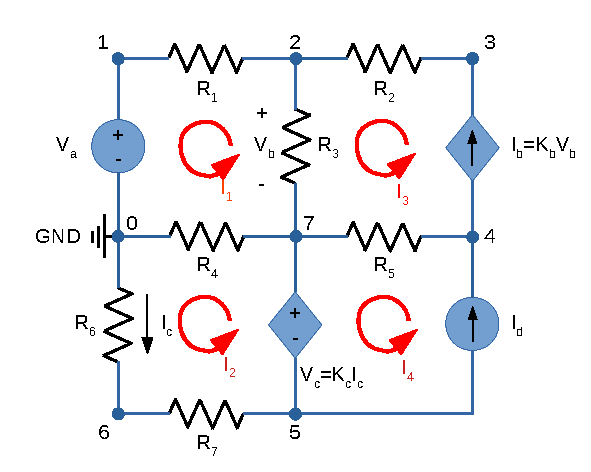
\includegraphics[width=0.7\linewidth]{MeshMethod.pdf}
  \caption{Mesh Currents Identification}
  \label{fig:MeshMethod}
\end{figure}

$$
\begin{cases}
  \text{Mesh 1: } R_{1}I_{1}+V_{a}+R_{4}(I_{1}-I_{2})+R_{3}(I_{1}-I_{3}) = 0\\
  \text{Mesh 2: } R_{4}(I_{2}-I_{1})+R_{6}I_{2}+R_{7}I_{2}-K_{c}I_{2} = 0\\
  \text{Current b: } I_{3} = I_{b} = K_{b}V_{b}\\
  \text{Current d: } I_{4} = I_{d}\\
  \\
  \text{Ohm's Law: } V_{b} = R_{3}(I_{3}-I_{1})
\end{cases}
$$
We can now present this same system in matrix form:
$$
\begin{bmatrix}
  R_{1}+R_{3}+R_{4} & -R_{4} & -R_{3} & 0 \\
  -R_{4} & R_{4}+R_{6}+R_{7}-K_{c} & 0 & 0\\
  R_{3}K_{b} & 0 & 1-K_{b}R_{3} & 0\\
  0 & 0 & 0 & 1
\end{bmatrix}
=
\begin{bmatrix}
  I_{1}\\
  I_{2}\\
  I_{3}\\
  I_{4}
\end{bmatrix}
\begin{bmatrix}
  -V_{a}\\
  0\\
  0\\
  I_{d}
\end{bmatrix}
$$
Solving the system above, one can determine the current in each mesh, and from there compute each of the currents and voltages in the circuit.


\subsection{Node Method}
\label{subsec:Node Method}\par
The Node Method consists on applying KCL in nodes not connected to voltage sources. In doing so, one can find a set of linnearly independent equations that represent the circuit. However, the number of unknows will be greater then the number of equations, because some nodes are connected to voltage sources. In order to find more equations, one can find relations between the currents imposed by the current sources and the currents in each branch. Beyond, this relations it is also necessary to use Ohm's Law.\par
The identification of the directions of the currents is shown bellow in Figure \ref{fig:NodeMethod}:


\begin{figure}[h] \centering
  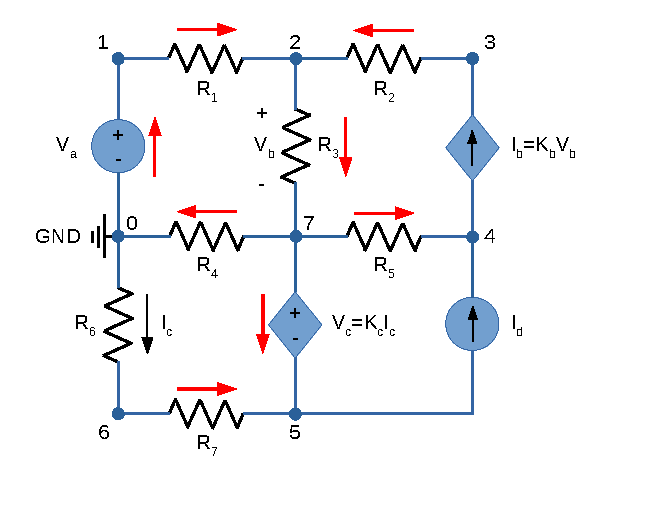
\includegraphics[width=0.7\linewidth]{NodeMethod.pdf}
  \caption{Currents Direction Identification}
  \label{fig:NodeMethod}
\end{figure}

Now one can set a system of linnearly independent equations:
$$
\begin{cases}
  \text{Node 1: } V_{1} = V_{a}\\
  \text{Node 2: } G_{1}(V_{1}-V_{2})+G_{2}(V_{3}-V_{2})-G_{3}(V_{2}-V_{7}) = 0\\
  \text{Node 3: } -G_{2}(V_{3}-V_{2})+K_bV_{b} = 0\\
  \text{Node 4: } G_{5}(V_{7}-V_{4})+I_{d}-K_bV_{b} = 0\\
  \text{Node 5: } V_{c}=V_{7}-V_{5}\\
  \text{Node 6: } G_{6}(V_{0}-V_{6})-G_{7}(V_{6}-V_{5}) = 0\\
  \text{Node 7: } G_{4}(V_{7}-V_{0})+G_{5}(V_{7}-V_{4})+I_{x}-G_{3}(V_{2}-V_{7}) = 0\\
  \\
  \text{Current x: } I_{x} = I_{d}-I_{c}\\
  \text{Current c: } I_{c} = G_{6}(0-V_{6})\\
  \text{Voltage b: } V_{b} = V_{2}-V_{7}
\end{cases}
$$
Writing the equations above in matricial form, one gets:
$$
\begin{bmatrix}
  1 & 0 & 0 & 0 & 0 & 0 & 0\\
  G_{1} & -G_{1}-G_{2}-G_{3} & G_{2} & 0 & 0 & 0 & G_{3}\\
  0 & G_{2}+K_{b} & -G_{2} & 0 & 0 & 0 & -K_{b}\\
  0 & -K_{b} & 0 & -G_{5} & 0 & 0 & G_{5}+K_{b}\\
  0 & 0 & 0 & 0 & -1 & K_{c}G_{6} & 1\\
  0 & 0 & 0 & 0 & G_{7} & -G_{6}-G_{7} & 0\\
  0 & G_{3} & 0 & G_{5} & 0 & -G_{6} & -G_{3}-G_{4}-G_{5}
\end{bmatrix}
=
\begin{bmatrix}
  V_{1}\\
  V_{2}\\
  V_{3}\\
  V_{4}\\
  V_{5}\\
  V_{6}\\
  V_{7}
\end{bmatrix}
\begin{bmatrix}
  V_{a}\\
  0\\
  0\\
  -I_{d}\\
  0\\
  0\\
  I_{d}
\end{bmatrix}
$$\par
Solving this system, one obtains the voltage drops between each branch and the ground branch. Therefore, it is possible complete the circuit analysis.

\underline{Note}: The results obtained in the Mesh Method must be the same as the results obtained in the Node Method.\par

The circuit analysis results are shown in the next subsection (\ref{subsec:Theoretical Analysis Results}).


\subsection{Theoretical Analysis Results}
\label{subsec:Theoretical Analysis Results}
\begin{table} [H]
  \centering
  \begin{tabular}{|l|r|}
    \hline    
    {\bf Name} & {\bf Value [A or V]} \\ \hline
    I_b & -0.000226\\ \hline
I_d & 0.001012\\ \hline
I_{R1} & 0.000216\\ \hline
I_{R2} & -0.000226\\ \hline
I_{R3} & -0.000010\\ \hline
I_{R4} & 0.001195\\ \hline
I_{R5} & -0.001238\\ \hline
I_{R6} & 0.000978\\ \hline
I_{R7} & 0.000978\\ \hline
V_1 & 5.125627\\ \hline
V_2 & 4.903891\\ \hline
V_3 & 4.446215\\ \hline
V_4 & 8.768409\\ \hline
V_5 & -2.982745\\ \hline
V_6 & -1.975719\\ \hline
V_7 & 4.934963\\ \hline

  \end{tabular}
  \caption{Operating point. A variable preceded by @ is of type {\em current}
    and expressed in Ampere; other variables are of type {\it voltage} and expressed in
    Volt.}
  \label{tab:op_analysis}
\end{table}


